\subsection{Fragmentation}
    \subsubsection*{Problems}
    \begin{enumerate}[label=\bfseries Problem \arabic*:,leftmargin=*,labelindent=1em]
    %addto counter에 앞서 subsection의 문제 개수만큼 적으면 자동으로 counting
    %image 번호만 신경써주면 된다.
    \addtocounter{enumi}{8}
    %%%%%%%%%%%%%%%%%%%%%%%%%%%%%%%%%%%%%%%%%%%%%%%%% Problem 3-9
        \item Find the first IP datagram containing the first part of the segment sent to 128.119.245.12 sent by your computer via the traceroute command to gaia.cs.umass.edu, after you specified that the traceroute packet length should be 3000. Has that segment been fragmented across more than one IP datagram?\\[0.2mm]
        \soln Yes, the segment is fragmented into 3 IP datagrams.
    %     \vspace{-4mm}  
        \begin{figure}[!h]\centering
        \hspace{15mm}  
    		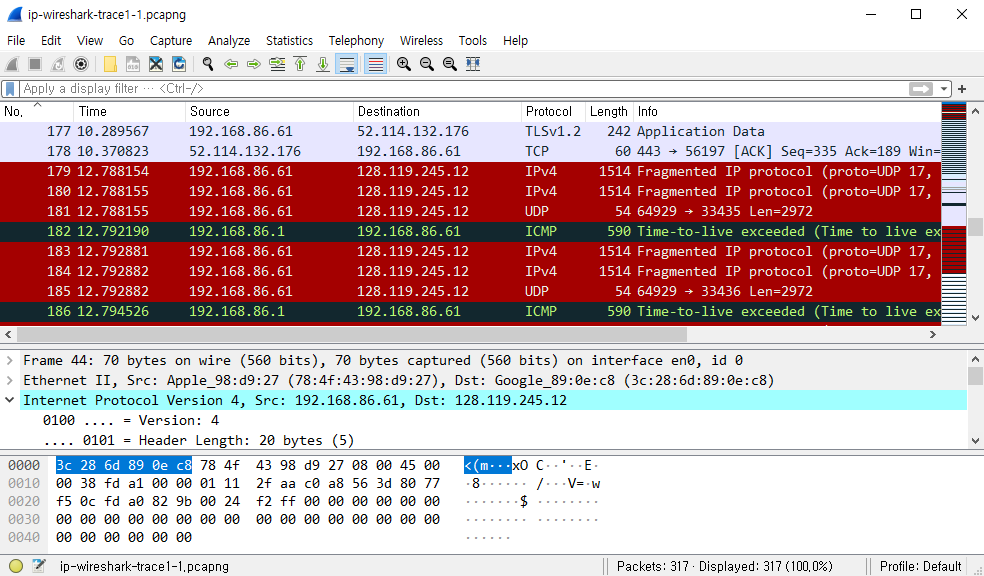
\includegraphics[width=.85\textwidth]{image/week02/3-9-1.png}
    		\caption{\footnotesize Problem 3-9's screenshot : }
    		\vspace{-10pt}
        \end{figure}
    %%%%%%%%%%%%%%%%%%%%%%%%%%%%%%%%%%%%%%%%%%%%%%%%% Problem 3-10
        \item What information in the IP header indicates that this datagram been fragmented? \\[0.2mm]
        \soln Since the flags more fragments bit is ‘Set’, we know that this datagram has been fragmented.
    %     \vspace{-4mm}  
\clearpage
        \begin{figure}[!h]\centering
        \hspace{15mm}  
    		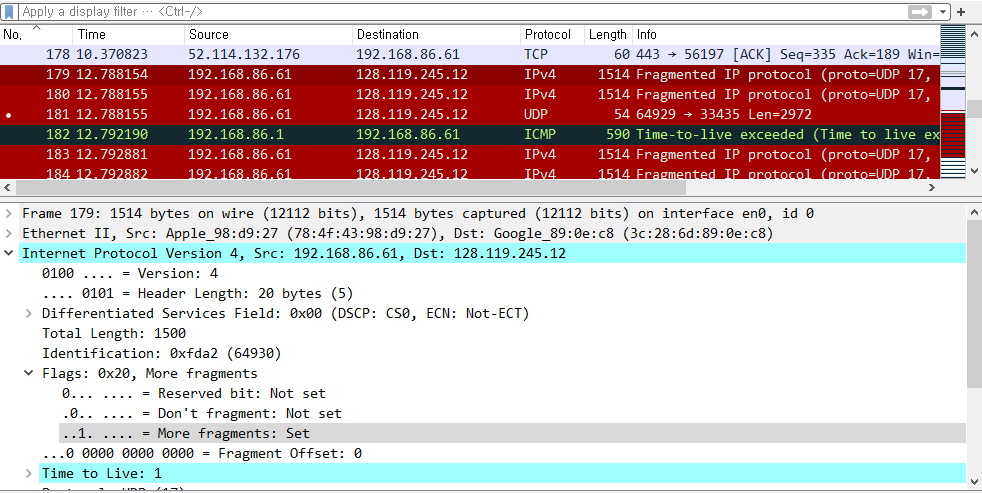
\includegraphics[width=.78\textwidth]{image/week02/3-a-1.png}
    		\caption{\footnotesize Problem 3-10's screenshot : }
    		\vspace{-10pt}
        \end{figure}
    %%%%%%%%%%%%%%%%%%%%%%%%%%%%%%%%%%%%%%%%%%%%%%%%% Problem 3-11
        \item What information in the IP header for this packet indicates whether this is the first fragment versus a latter fragment?\\[0.2mm]
        \soln Since the fragment offset is 0, we know that this is the first fragment.
    %     \vspace{-4mm}  
        \begin{figure}[!h]\centering
        \hspace{15mm}  
    		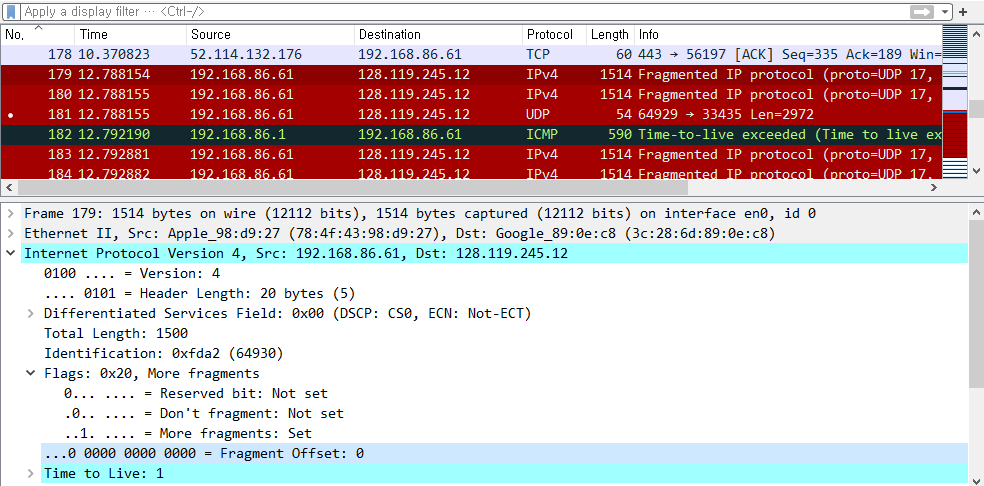
\includegraphics[width=.78\textwidth]{image/week02/3-b-1.png}
    		\caption{\footnotesize Problem 3-11's screenshot : }
    		\vspace{-10pt}
        \end{figure}
    %%%%%%%%%%%%%%%%%%%%%%%%%%%%%%%%%%%%%%%%%%%%%%%%% Problem 3-12
        \item How many bytes are there in is this IP datagram (header plus payload)?\\[0.2mm]
        \soln 1500 bytes
    %     \vspace{-4mm}  
        \begin{figure}[!h]\centering
        \hspace{15mm}  
    		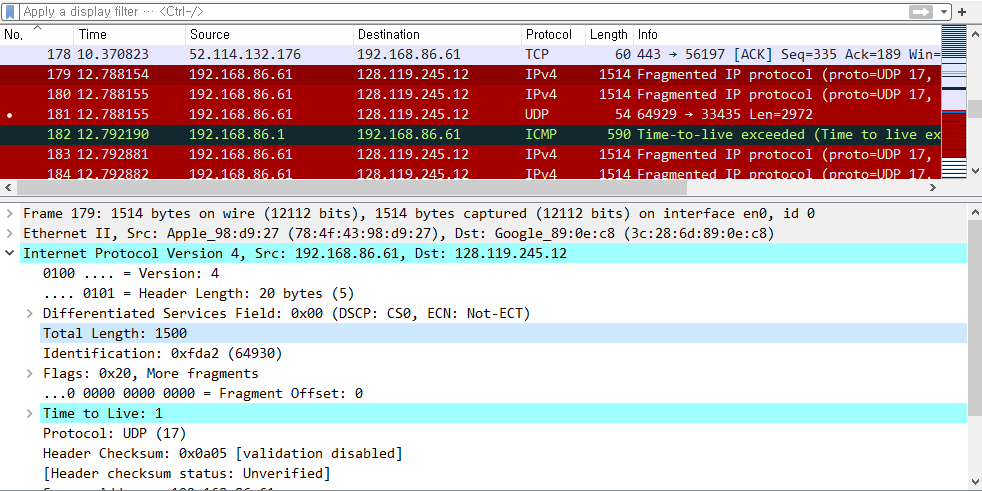
\includegraphics[width=.78\textwidth]{image/week02/3-c-1.png}
    		\caption{\footnotesize Problem 3-12's screenshot : }
    		\vspace{-10pt}
        \end{figure}
\newpage
    %%%%%%%%%%%%%%%%%%%%%%%%%%%%%%%%%%%%%%%%%%%%%%%%% Problem 3-13
        \item Now inspect the datagram containing the second fragment of the fragmented UDP segment. What information in the IP header indicates that this is not the first datagram fragment?\\[0.2mm]
        \soln Since the fragment offset is 1480, we know that this is not the first fragment.
    %     \vspace{-4mm}  
        \begin{figure}[!h]\centering
        \hspace{15mm}  
    		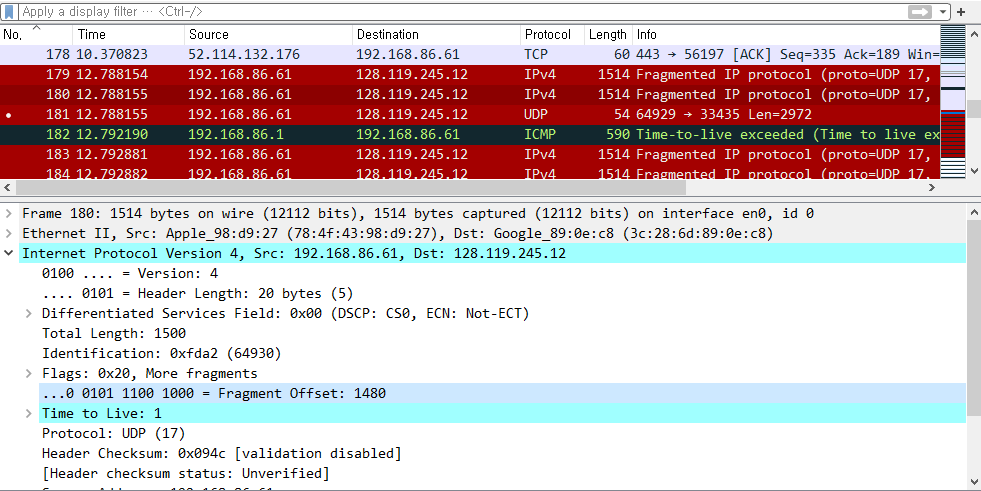
\includegraphics[width=.85\textwidth]{image/week02/3-d-1.png}
    		\caption{\footnotesize Problem 3-13's screenshot : }
    		\vspace{-10pt}
        \end{figure}
    %%%%%%%%%%%%%%%%%%%%%%%%%%%%%%%%%%%%%%%%%%%%%%%%% Problem 3-14
        \item What fields change in the IP header between the first and second fragment?\\[0.2mm]
        \soln Fragment offset and Header checksum
        \begin{figure}[h!]
        \centering
        \subfloat[ ]{
            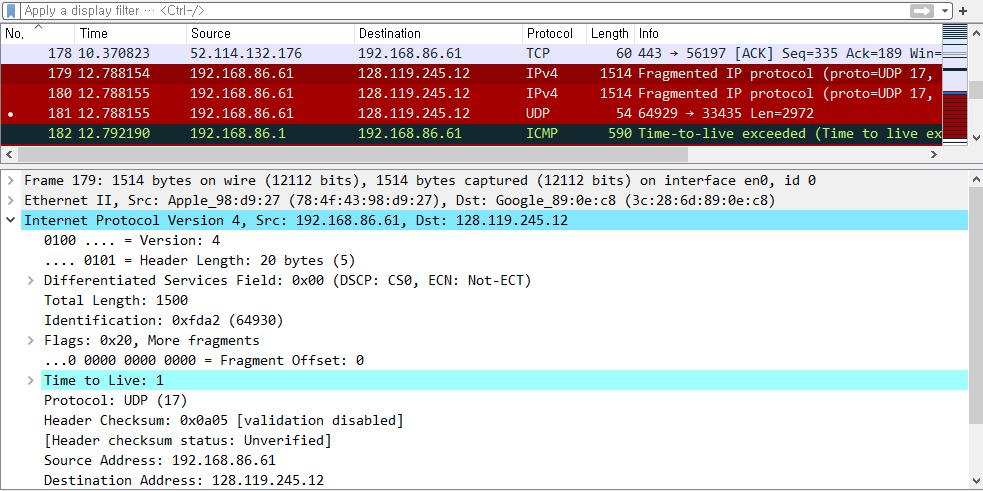
\includegraphics[width=0.48\textwidth] {image/week02/3-e-1.png}
        }\hspace{2mm}
        \subfloat[ ]{
            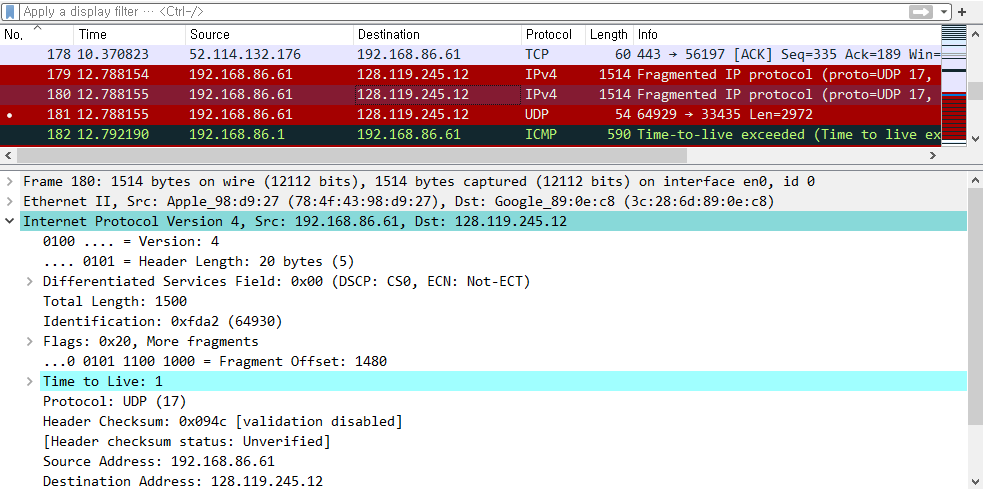
\includegraphics[width=0.48\textwidth] {image/week02/3-e-2.png}
        }\caption{\footnotesize Problem 3-14's screenshot : }
        \end{figure}
    %     \vspace{-4mm}  
    %     \begin{figure}[!h]\centering
    %     \hspace{15mm}  
    % 		\includegraphics[width=.85\textwidth]{image/week02/ }
    % 		\caption{\footnotesize Problem 3-14's screenshot : }
    % 		\vspace{-10pt}
    %     \end{figure}
    \end{enumerate}
\newpage